\documentclass[a4paper]{article} 

\usepackage{graphicx}
\addtolength{\hoffset}{-2.25cm}
\addtolength{\textwidth}{4.5cm}
\addtolength{\voffset}{-3.25cm}
\addtolength{\textheight}{5cm}
\setlength{\parskip}{0pt}
\setlength{\parindent}{0in}

%----------------------------------------------------------------------------------------
%	PACKAGES AND OTHER DOCUMENT CONFIGURATIONS
%----------------------------------------------------------------------------------------

\usepackage{blindtext} % Package to generate dummy text
\usepackage{charter} % Use the Charter font
\usepackage[utf8]{inputenc} % Use UTF-8 encoding
\usepackage{microtype} % Slightly tweak font spacing for aesthetics
\usepackage[english, ngerman]{babel} % Language hyphenation and typographical rules
\usepackage{amsthm, amsmath, amssymb} % Mathematical typesetting
\usepackage{float} % Improved interface for floating objects
\usepackage[final, colorlinks = true, 
            linkcolor = black, 
            citecolor = black]{hyperref} % For hyperlinks in the PDF
\usepackage{graphicx, multicol} % Enhanced support for graphics
\usepackage{xcolor} % Driver-independent color extensions
\usepackage{marvosym, wasysym} % More symbols
\usepackage{rotating} % Rotation tools
\usepackage{censor} % Facilities for controlling restricted text
\usepackage{listings, style/lstlisting} % Environment for non-formatted code, !uses style file!
\usepackage{pseudocode} % Environment for specifying algorithms in a natural way
\usepackage{style/avm} % Environment for f-structures, !uses style file!
\usepackage{booktabs} % Enhances quality of tables
\usepackage{tikz-qtree} % Easy tree drawing tool
\tikzset{every tree node/.style={align=center,anchor=north},
         level distance=2cm} % Configuration for q-trees
\usepackage{style/btree} % Configuration for b-trees and b+-trees, !uses style file!
\usepackage[backend=biber,style=numeric,
            sorting=nyt]{biblatex} % Complete reimplementation of bibliographic facilities
\addbibresource{ecl.bib}
\usepackage{csquotes} % Context sensitive quotation facilities
\usepackage[yyyymmdd]{datetime} % Uses YEAR-MONTH-DAY format for dates
\renewcommand{\dateseparator}{-} % Sets dateseparator to '-'
\usepackage{fancyhdr} % Headers and footers
\pagestyle{fancy} % All pages have headers and footers
\fancyhead{}\renewcommand{\headrulewidth}{0pt} % Blank out the default header
\fancyfoot[L]{} % Custom footer text
\fancyfoot[C]{} % Custom footer text
\fancyfoot[R]{\thepage} % Custom footer text
\newcommand{\note}[1]{\marginpar{\scriptsize \textcolor{red}{#1}}} % Enables comments in red on margin

%----------------------------------------------------------------------------------------

\usepackage{subcaption}
\usepackage[T1]{fontenc}
\usepackage[utf8]{inputenc}
\usepackage{lmodern}

\usepackage{minted}

\begin{document}

%-------------------------------
%	TITLE SECTION
%-------------------------------
\fancyhead[C]{}
\hrule \medskip % Upper rule
\begin{minipage}{0.295\textwidth} 
\raggedright
\footnotesize
Huang Hua \hfill\\   
\textbf{}\\
Haixu Wang\hfill\\

\end{minipage}
\begin{minipage}{0.4\textwidth} 
\centering 
\large 
Homework Assignment 1\\ 
\end{minipage}
\begin{minipage}{0.295\textwidth} 
\raggedleft
\today\hfill\\
\end{minipage}
\medskip\hrule 
\bigskip

%-------------------------------
%	CONTENTS
%-------------------------------

\section{Decision Tree}
In this assignment, we use xgboost and scikit-learn packages in python to train the datasets separately. Since we don't have labels in test data sets, we have to use valid datasets as test datasets. The scikit-learn DecisionTreeClassifier package has two main splitting criterion: Gini and Entropy. Here, we use entropy as splitting criterion following the lecture notes.
\subsection{Madelon Dataset}
\begin{table}[H]
\centering
\caption{Data information}
\begin{tabular}{|c|c|c|c|}
	\hline
	Dataset & Features &\textbf{Train\_obs} & \textbf{Test\_obs}\\
	\hline
    Madelon & 500 & 2000 & 600\\
	\hline
\end{tabular}
\end{table}
In this dataset, this dataset has 500 features. We have 2000 observations as training data. Figure 1 shows after depth=5, the model from xgboost over fits the training data. And the error of test data converges to 0.15. The optimal choice of depth is 3 0r 4.
\begin{figure}[h]
  	\centering
  	\begin{subfigure}[b]{0.3\linewidth}
  	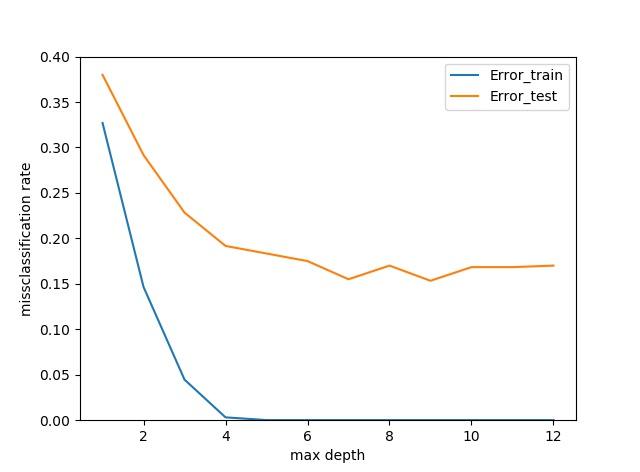
\includegraphics[width=\textwidth]{madelon_result.jpeg}
	\caption{Results from xgboost}
	\end{subfigure}
	
    \begin{subfigure}[b]{0.3\linewidth}
    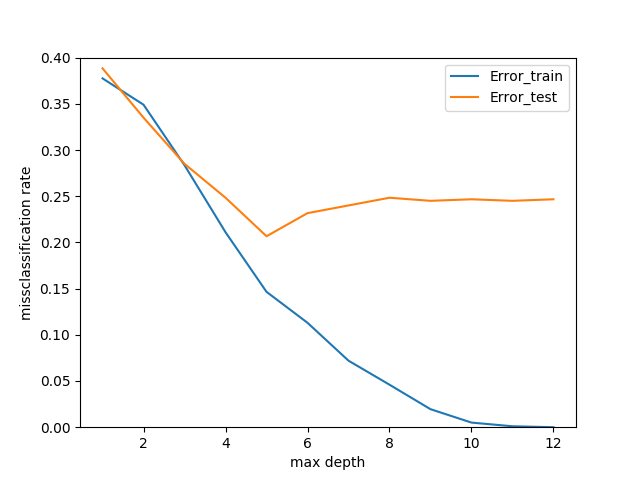
\includegraphics [width=\linewidth]{madelon.png}
    \caption{Results from Scikit\--learn}
    \end{subfigure}

\caption{Results for dataset Madelon}

	\label{fig1}
\end{figure}

\begin{table}[H]
\centering
\caption{Test error with depth}
\begin{tabular}{|c|c|}
	\hline
	Testerror & Tree depth \\
	\hline
	0.38 & 1\\
	\hline
	0.292 &2\\
	\hline
	0.228 &3\\
	\hline
     0.192 &4\\
     \hline
     0.183 & 5\\
     \hline
     0.175& 6\\
     \hline
     0.155& 7\\
     \hline
     0.17 & 8\\
     \hline
     0.153 & 9\\
     \hline
     0.1683 & 10\\
     \hline
     0.168 & 11\\
     \hline
     0.17 & 12 \\
	\hline
\end{tabular}
\end{table}

\subsection{Wilt Dataset}
\begin{table}[H]
\centering
\caption{Data information}
\begin{tabular}{|c|c|c|c|}
	\hline
	Dataset & Features &\textbf{Train\_obs} & \textbf{Test\_obs}\\
	\hline
    Wilt & 5 & 4339 & 500\\
	\hline
\end{tabular}
\end{table}
In this dataset, there are only 5 features but 4339 observations. After depth=2, the model from xgboost over fits the training data. And the error of test data converges to 0.18. The optimal choice of depth is 7.
\begin{figure}[h]
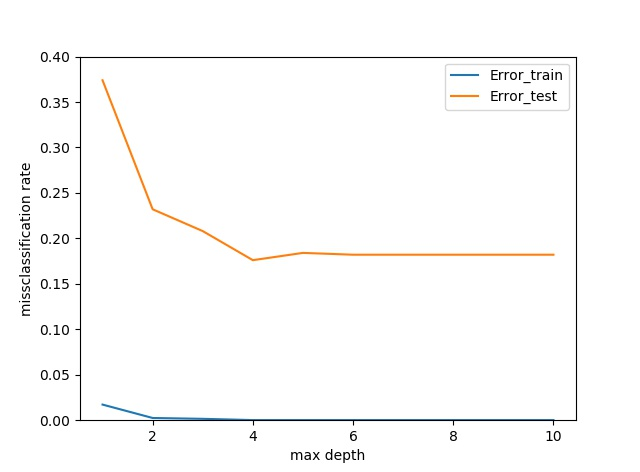
\includegraphics[width=\textwidth]{wilt_result.jpeg}
\caption{}
\label{fig3}
\end{figure}

\begin{table}[H]
\centering
\caption{Test error with depth}
\begin{tabular}{|c|c|}
	\hline
	Testerror & Tree depth \\
	\hline
	0.374 & 1\\
	\hline
	0.232 &2\\
	\hline
	0.208 &3\\
	\hline
     0.176 &4\\
     \hline
     0.184 & 5\\
     \hline
     0.182& 6\\
     \hline
     0.182& 7\\
     \hline
     0.182 & 8\\
     \hline
     0.182 & 9\\
     \hline
     0.182 & 10\\
	\hline
\end{tabular}
\end{table}

\subsection{Gisette Dataset}
\begin{table}[h]
\centering
\caption{Data information}
\begin{tabular}{|c|c|c|c|}
	\hline
	Dataset & Features &\textbf{Train\_obs} & \textbf{Test\_obs}\\
	\hline
    Gisette & 5000 & 6000 & 1000\\
	\hline
\end{tabular}
\end{table}
First of all, in this dataset, we have too many features and relative small observations. With decision tree algorithm in xgboost, after depth=4, we can see the model over fits the training data. Therefore, the optimal choice of depth is 4. 
\begin{figure}[h]
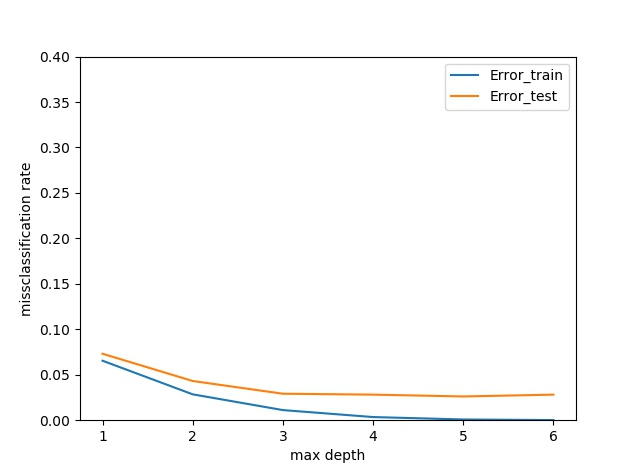
\includegraphics[width=\textwidth]{gisette_result.jpeg}
\caption{}
\label{}
\end{figure}
\begin{table}[H]
\centering
\caption{Test error with depth}
\begin{tabular}{|c|c|}
	\hline
	Testerror & Tree depth \\
	\hline
	0.073 & 1\\
	\hline
	0.043 &2\\
	\hline
	0.029 &3\\
	\hline
     0.028 &4\\
     \hline
     0.026 & 5\\
     \hline
     0.028& 6\\
	\hline
\end{tabular}
\end{table}

\bigskip

%------------------------------------------------

\section{Code}
\begin{minted}{c}
def clearall():
    all = [var for var in globals() if (var[:2], var[-2:]) != ("__", "__")]
    for var in all:
        del globals()[var] 
        
clearall()

import xgboost as xgb
import numpy as np
from xgboost import XGBClassifier
from sklearn import tree
from sklearn.model_selection import train_test_split
from sklearn.metrics import accuracy_score
import pandas as pd
import matplotlib.pyplot as plt

def decision_tree(X, Y, XTest, YTest, maxDepth):
    rateTrain=np.zeros(maxDepth.shape[0])
    rateTest=np.zeros(maxDepth.shape[0])
    for i in range(maxDepth.shape[0]):
        #fit model no training data
        #clf=tree.DecisionTreeClassifier(criterion='entropy',max_depth=maxDepth[i])     
        clf=XGBClassifier(max_depth=maxDepth[i])
        clf.fit(X,Y)
        print(clf)
        y=clf.predict(X)
        yTest=clf.predict(XTest)
        py = [round(value) for value in y]
        pyTest = [round(value) for value in yTest]
        rateTrain[i]=1-np.mean(py==Y)
        rateTest[i]=1-np.mean(pyTest==YTest)    
        accuracy=accuracy_score(pyTest,YTest)
        print("Accuracy:%.2f%%"%(accuracy*100.0))
        print('train, test misclassification error: ', rateTrain[i],
                rateTest[i])
    return rateTrain, rateTest

def problem_1a():
    #load data
    dmd=np.loadtxt('E:\study material\FSU\Fall2018\ML\AML_Fall2018\Data\MADELON\madelon_train.txt')
    dmdl=np.genfromtxt('E:\study material\FSU\Fall2018\ML\AML_Fall2018\Data\MADELON\madelon_trainlabels.txt')
    dmdv=np.loadtxt('E:\study material\FSU\Fall2018\ML\AML_Fall2018\Data\MADELON\madelon_valid.txt')
    dmdlv=np.loadtxt('E:\study material\FSU\Fall2018\ML\AML_Fall2018\Data\MADELON\madelon_validlabels.txt')
    
    maxDepth=np.arange(12)+1
    train, test=decision_tree(dmd, dmdl, dmdv, dmdlv, maxDepth)
    
    figureIndex=0
    plt.figure(figureIndex)
    figureIndex += 1
    plt.plot(maxDepth, train, label='Error_train')
    plt.plot(maxDepth, test,  label='Error_test')

    plt.xlabel('max depth')
    plt.ylabel('missclassification rate')
    plt.ylim([0, 0.4])
    plt.legend()
    plt.show()

def problem_1b():
    X=np.genfromtxt('E:\study material\FSU\Fall2018\ML\AML_Fall2018\Data\wilt\wilt_train.csv', delimiter=',')
    Y=np.loadtxt('E:\study material\FSU\Fall2018\ML\AML_Fall2018\Data\wilt\wilt_trainlabels.txt')
    XTest=np.genfromtxt('E:\study material\FSU\Fall2018\ML\AML_Fall2018\Data\wilt\wilt_test.csv', delimiter=',')
    YTest=np.loadtxt('E:\study material\FSU\Fall2018\ML\AML_Fall2018\Data\wilt\wilt_testlabels.txt')
    maxDepth=np.arange(10)+1
    train, test=decision_tree(X, Y, XTest, YTest, maxDepth)
    
    figureIndex=0
    plt.figure(figureIndex)
    figureIndex += 1
    plt.plot(maxDepth, train, label='Error_train')
    plt.plot(maxDepth, test,  label='Error_test')

    plt.xlabel('max depth')
    plt.ylabel('missclassification rate')
    plt.ylim([0, 0.4])
    plt.legend()
    plt.show()
    
def problem_1c():
    X=np.loadtxt('E:\study material\FSU\Fall2018\ML\AML_Fall2018\Data\Gisette\gisette_train.txt')
    Y=np.loadtxt('E:\study material\FSU\Fall2018\ML\AML_Fall2018\Data\Gisette\gisette_trainlabels.txt')
    XTest=np.loadtxt('E:\study material\FSU\Fall2018\ML\AML_Fall2018\Data\Gisette\gisette_valid.txt')
    YTest=np.loadtxt('E:\study material\FSU\Fall2018\ML\AML_Fall2018\Data\Gisette\gisette_validlabels.txt')
    maxDepth=np.arange(6)+1
    train, test=decision_tree(X, Y, XTest, YTest, maxDepth)
    
    figureIndex=0
    plt.figure(figureIndex)
    figureIndex += 1
    plt.plot(maxDepth, train, label='Error_train')
    plt.plot(maxDepth, test,  label='Error_test')

    plt.xlabel('max depth')
    plt.ylabel('missclassification rate')
    plt.ylim([0, 0.4])
    plt.legend()
    plt.show()
    

problem_1a()
#problem_1b()
#problem_1c()
\end{minted}
\bigskip

%------------------------------------------------

\end{document}
